%%%%%%%%%%%%%%%%%%%%%%%%%%%%%%%%%%%%%%%%%%%%%%%%%%%%%%%%%%%
\begin{frame}
  \begin{center}
    {\Large Use of Deep Learning in NLP}
  \end{center}
\end{frame}


%%%%%%%%%%%%%%%%%%%%%%%%%%%%%%%%%%%%%%%%%%%%%%%%%%%%%%%%%%%
\begin{frame}[fragile]\frametitle{Quiz Time!}
Which is human? Which is machine? Both by?
\begin{center}
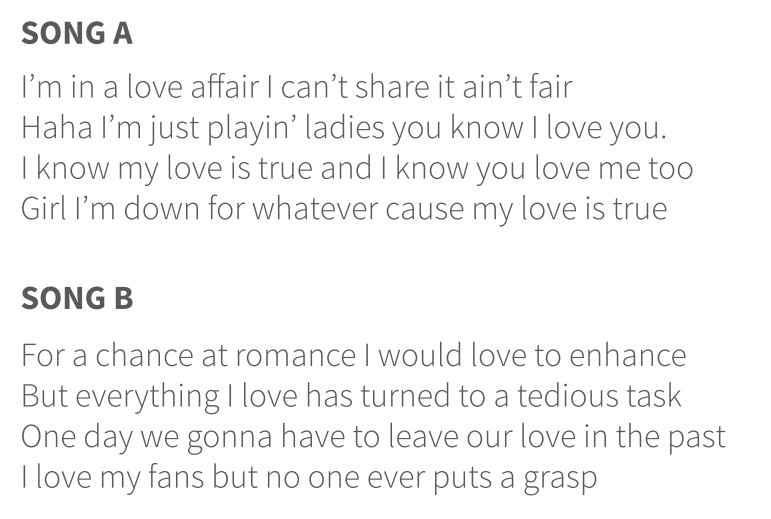
\includegraphics[width=0.9\linewidth,keepaspectratio]{dnlp}

%\tiny{(Ref:  DeepBeat.org - Online tool for rap lyrics generator)}
\end{center}
\end{frame}

%%%%%%%%%%%%%%%%%%%%%%%%%%%%%%%%%%%%%%%%%%%%%%%%%%%%%%%%%%%
\begin{frame}[fragile]\frametitle{Quiz Time!}
Answer: Both.
\begin{center}
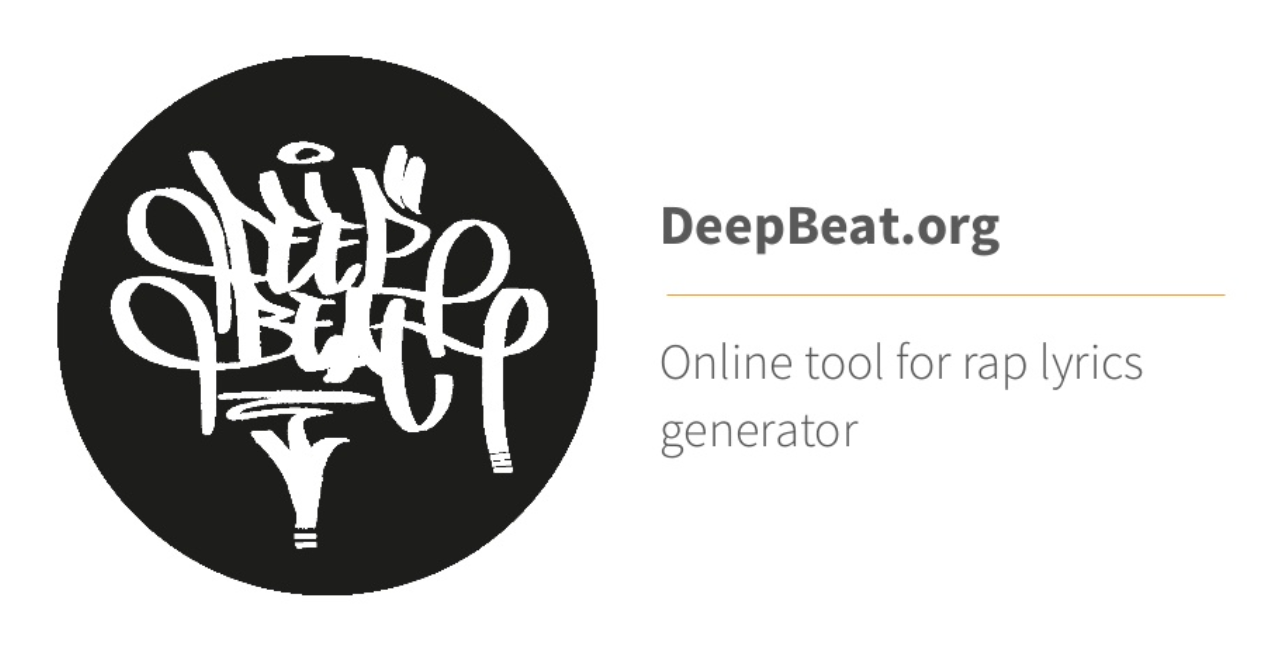
\includegraphics[width=0.5\linewidth,keepaspectratio]{deepbeat}

	\begin{itemize}
	\item Eric Malmi: mines past rap songs and generates a new one based on similar rhymes and keywords, line by line.
	\item Start with a line from one rap lyric and ask the computer to search through the database for another line on the same topic that best rhymes. It then repeats this process for the next line and so on.
	\item Reference: ``DopeLearning: A Computational Approach to Rap Lyrics Generation'' (http://arxiv.org/pdf/1505.04771v1.pdf)
	\end{itemize}
\end{center}
\end{frame}


%%%%%%%%%%%%%%%%%%%%%%%%%%%%%%%%%%%%%%%%%%%%%%%%%%%%%%%%%%%
\begin{frame}[fragile]\frametitle{Turing Test}

A human judge engages in a natural language conversation with two other parties, one a human and the other a machine; if the judge cannot reliably tell which is which, then the machine is said to pass the test. 

\begin{center}
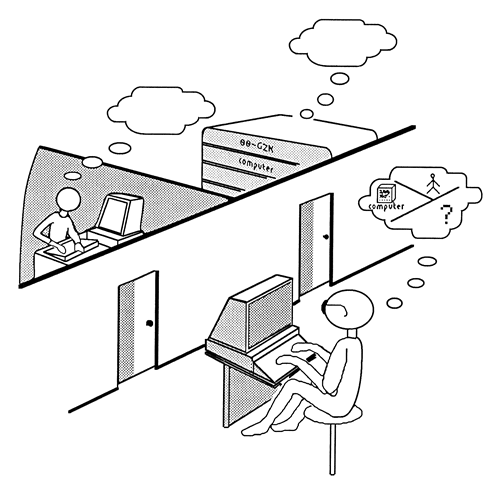
\includegraphics[width=0.4\linewidth,keepaspectratio]{turing}
\end{center}

Use of Deep Learning in Natural Language Processing is helping beat the Turing test, a mark of intelligence, ie Artifical Intelligence.
\end{frame}

%%%%%%%%%%%%%%%%%%%%%%%%%%%%%%%%%%%%%%%%%%%%%%%%%%%%%%%%%%%
\begin{frame}[fragile]\frametitle{NLP-AI}
	\begin{itemize}
	\item Natural Language Processing (Understanding-Generation) is an AI-Complete problem
	\item Most difficult AI problems are informally known as AI-complete or AI-hard 
	\item To call a problem AI-complete reflects an attitude that it would not be solved by a simple specific algorithm.
	\end{itemize}

\tiny{(Ref: https://en.wikipedia.org/wiki/AI-complete)}
\end{frame}

%%%%%%%%%%%%%%%%%%%%%%%%%%%%%%%%%%%%%%%%%%%%%%%%%%%%%%%%%%%
\begin{frame}[fragile]\frametitle{NLP Tasks}
	\begin{itemize}
	\item Part Of Speech Tagging: Assign part-of-speech to each word.
	\item Named Entity Recognition: Recognize people, places, etc. in a sentence.
	\item Language Modeling: Predict next word, Generate natural sentences.
	\item Translation:  Translate a sentence into another language.
	\item  Summarization: Summarize a paragraph in new words.
	\end{itemize}

\tiny{(Ref: How Deep Learning Quietly Revolutionized NLP - Lukasz Kaiser, Google Brain)}
\end{frame}

%%%%%%%%%%%%%%%%%%%%%%%%%%%%%%%%%%%%%%%%%%%%%%%%%%%%%%%%%%%
\begin{frame}[fragile]\frametitle{Let's discuss}
	\begin{itemize}
	\item What is Deep Learning? 
	\item Why is it important?
	\item How to apply Deep Learning to Natural Language Processing?
	\end{itemize}

\tiny{(Ref (next few slides):  Deep Learning for Natural Langauge Processing - Sihem Romdhani)}

\end{frame}



%%%%%%%%%%%%%%%%%%%%%%%%%%%%%%%%%%%%%%%%%%%%%%%%%%%%%%%%%%%
\begin{frame}[fragile]\frametitle{Machine Learning}
\begin{center}
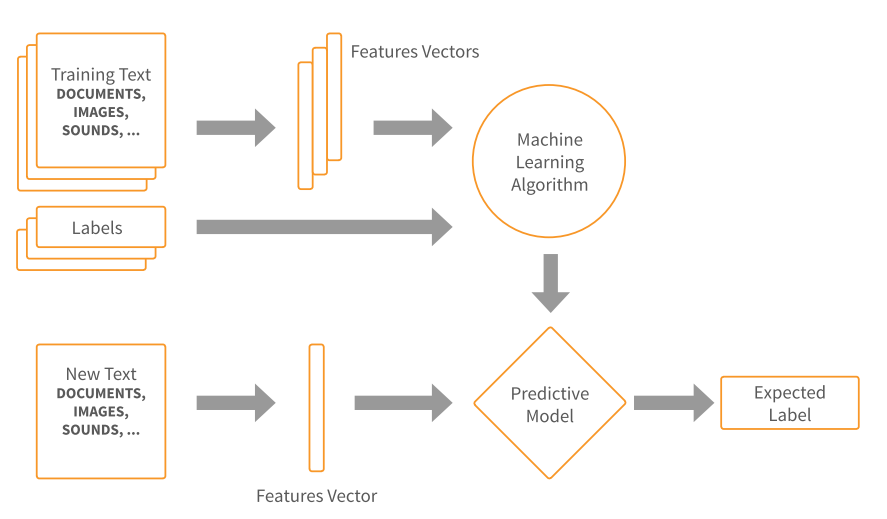
\includegraphics[width=0.8\linewidth,keepaspectratio]{dnlp1}

\tiny{(Ref:  Deep Learning for Natural Language Processing - Sihem Romdhani)}
\end{center}

Hand crafted features are needed in Machine Learning. E.g. for Spam Detection, features could be presennce of BIG \$ amounts, FROM country, etc.
\end{frame}

%%%%%%%%%%%%%%%%%%%%%%%%%%%%%%%%%%%%%%%%%%%%%%%%%%%%%%%%%%%
\begin{frame}[fragile]\frametitle{Deep Learning}
\begin{center}
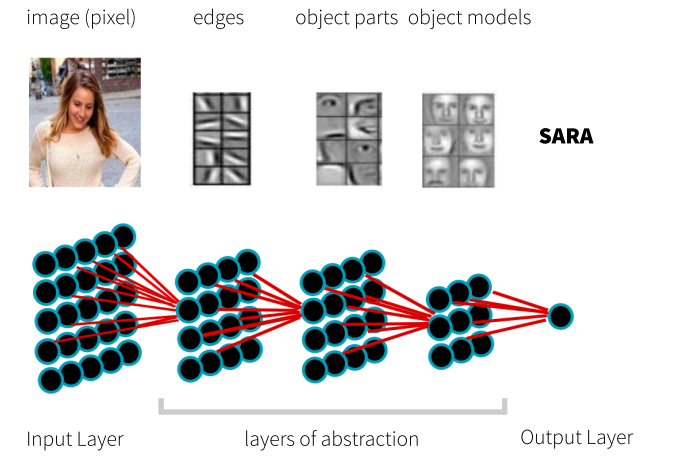
\includegraphics[width=0.6\linewidth,keepaspectratio]{dnlp2}

\tiny{(Ref:  Deep Learning for Natural Language Processing - Sihem Romdhani)}
\end{center}

Hand crafted features are NOT needed in Deep Learning. E.g. for Object Detection, CNNs are come up with own features like, edges, parts, etc.
\end{frame}



%%%%%%%%%%%%%%%%%%%%%%%%%%%%%%%%%%%%%%%%%%%%%%%%%%%%%%%%%%%
\begin{frame}[fragile]\frametitle{Need numbers not words!!}
How can we represent words?
\begin{center}
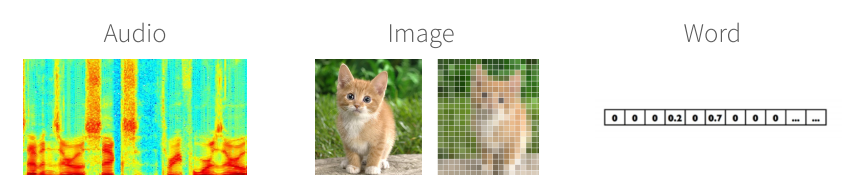
\includegraphics[width=0.8\linewidth,keepaspectratio]{dnlp3}

\tiny{(Ref:  Deep Learning for Natural Language Processing - Sihem Romdhani)}
\end{center}

Words, sentences, paragraphs, pages, documents, all need to represented by numbers, to be able to fed to ML/DL algorithm.
\end{frame}

%%%%%%%%%%%%%%%%%%%%%%%%%%%%%%%%%%%%%%%%%%%%%%%%%%%%%%%%%%%
\begin{frame}[fragile]\frametitle{Traditional methods to covert text to numeric}
With Vocabulary as the full set representing the whole corpus.
	\begin{itemize}
	\item Bag-of-Word: Count of occurrences of a word in a document
	\item  TF-IDF: Measures importance of a word in a document relative to the corpus
	\end{itemize}

\end{frame}

%%%%%%%%%%%%%%%%%%%%%%%%%%%%%%%%%%%%%%%%%%%%%%%%%%%%%%%%%%%
\begin{frame}[fragile]\frametitle{Challenges in traditional methods of encoding}
With Vocabulary as the full set representing the whole corpus.
	\begin{itemize}
	\item Sparse inputs
	\item   Context lost in encoding
	\end{itemize}

\begin{center}
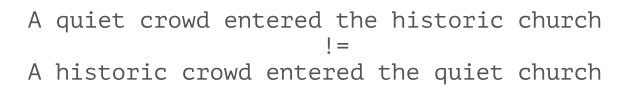
\includegraphics[width=0.8\linewidth,keepaspectratio]{dnlp9}

\tiny{(Ref:  Deep Learning for Natural Language Processing - Bargava,  Amit Kapoor)}
\end{center}

\end{frame}


%%%%%%%%%%%%%%%%%%%%%%%%%%%%%%%%%%%%%%%%%%%%%%%%%%%%%%%%%%%
\begin{frame}[fragile]\frametitle{Embeddings}
It just can not be any set of numbers representing words. Similar words should have similar numbers.

\begin{center}
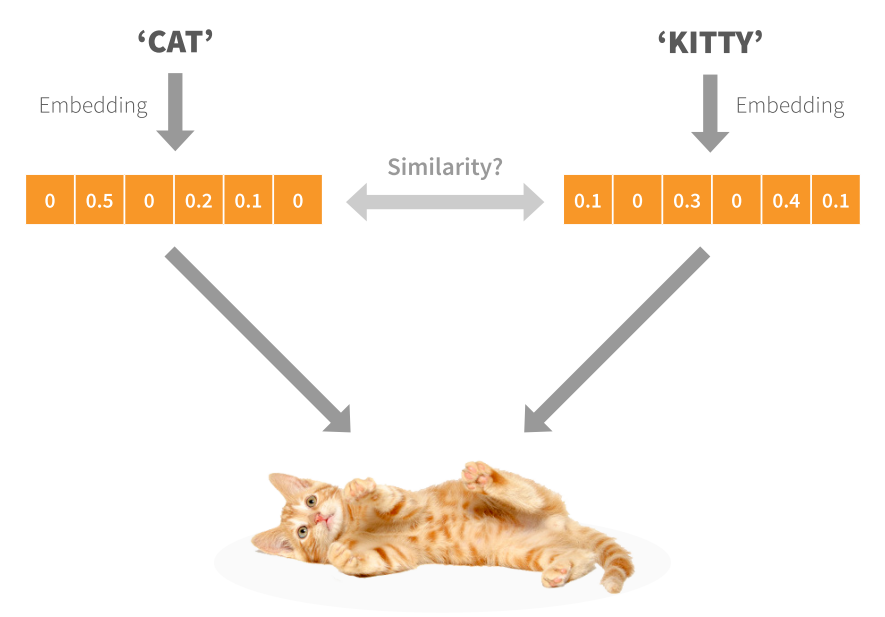
\includegraphics[width=0.6\linewidth,keepaspectratio]{dnlp4}

\tiny{(Ref:  Deep Learning for Natural Language Processing - Sihem Romdhani)}
\end{center}
\end{frame}


%%%%%%%%%%%%%%%%%%%%%%%%%%%%%%%%%%%%%%%%%%%%%%%%%%%%%%%%%%%
\begin{frame}[fragile]\frametitle{How to get good Embeddings?}
Context defines similarity

\begin{center}
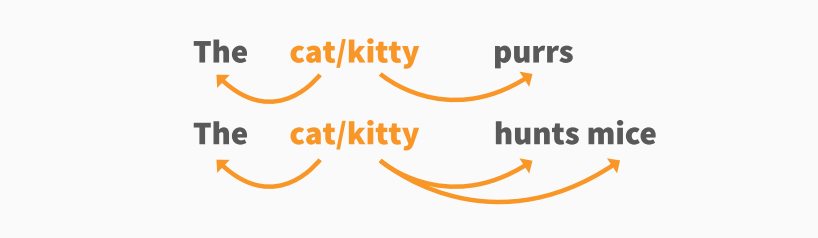
\includegraphics[width=0.6\linewidth,keepaspectratio]{dnlp5}

\tiny{(Ref:  Deep Learning for Natural Language Processing - Sihem Romdhani)}
\end{center}

Infer the meaning of words from the company they keep
\end{frame}

%%%%%%%%%%%%%%%%%%%%%%%%%%%%%%%%%%%%%%%%%%%%%%%%%%%%%%%%%%%
\begin{frame}[fragile]\frametitle{Word to Vector}
Context defines similarity

\begin{center}
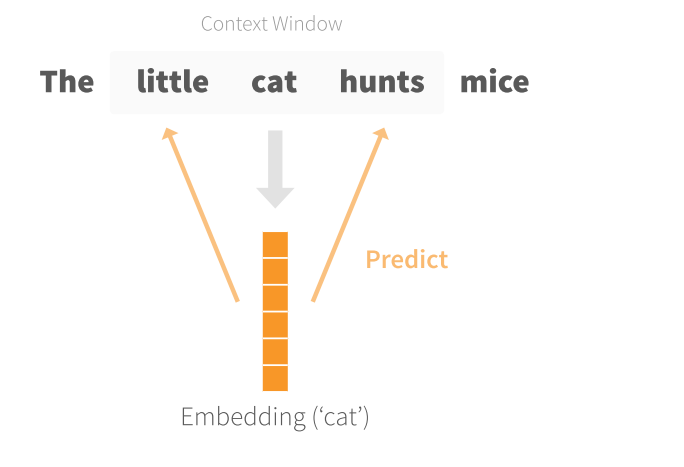
\includegraphics[width=0.6\linewidth,keepaspectratio]{dnlp6}

\tiny{(Ref:  Deep Learning for Natural Language Processing - Sihem Romdhani)}
\end{center}

Infer the meaning of words from the company they keep
\end{frame}

%%%%%%%%%%%%%%%%%%%%%%%%%%%%%%%%%%%%%%%%%%%%%%%%%%%%%%%%%%%
\begin{frame}[fragile]\frametitle{Word to Vector Examples}
Similar words are nearby

\begin{center}
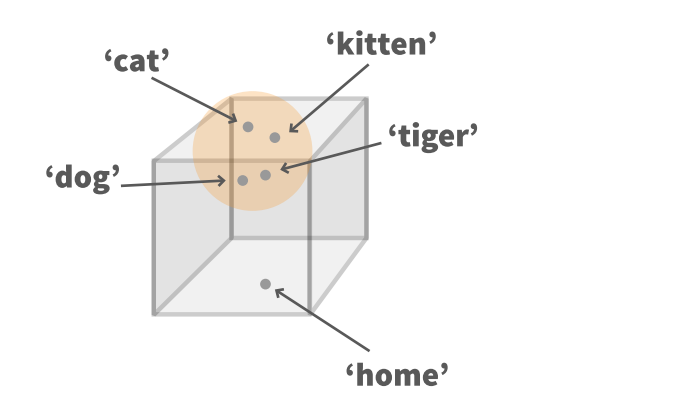
\includegraphics[width=0.6\linewidth,keepaspectratio]{dnlp7}

\tiny{(Ref:  Deep Learning for Natural Language Processing - Sihem Romdhani)}
\end{center}

Dissimilar words are away.
\end{frame}


%%%%%%%%%%%%%%%%%%%%%%%%%%%%%%%%%%%%%%%%%%%%%%%%%%%%%%%%%%%
\begin{frame}[fragile]\frametitle{Vector Algebra Possible}

\begin{center}
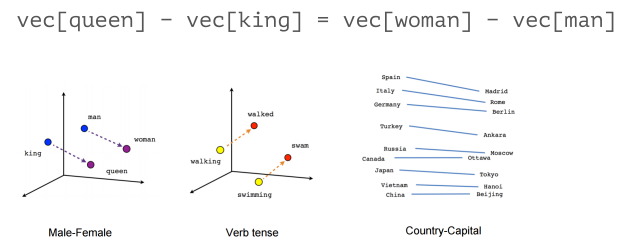
\includegraphics[width=\linewidth,keepaspectratio]{dnlp10}

\tiny{(Ref:   https://www.tensorflow.org/versions/r0.12/tutorials/word2vec/index.html)}
\end{center}

\end{frame}


%%%%%%%%%%%%%%%%%%%%%%%%%%%%%%%%%%%%%%%%%%%%%%%%%%%%%%%%%%%
\begin{frame}[fragile]\frametitle{Classifier}
Similar words are nearby

\begin{center}
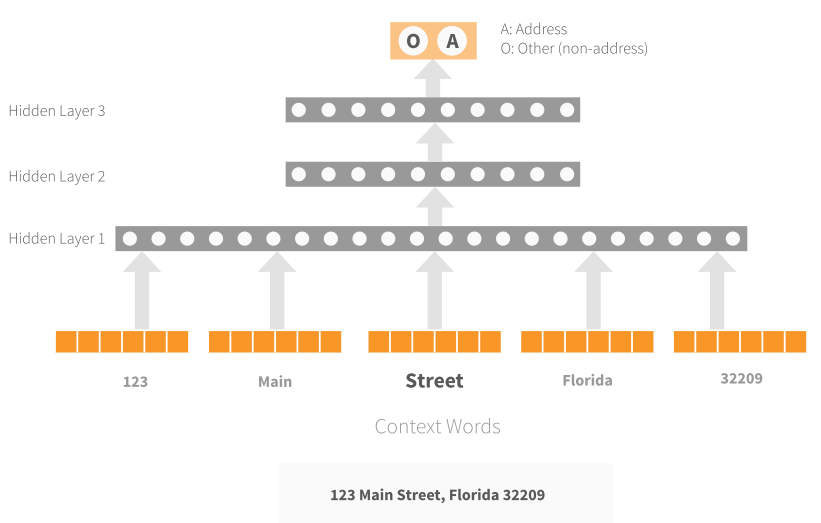
\includegraphics[width=0.6\linewidth,keepaspectratio]{dnlp8}

\tiny{(Ref:  Deep Learning for Natural Language Processing - Sihem Romdhani)}
\end{center}

Here ``Street''  is in the context of an Address, thus gets classified that way.
\end{frame}

%%%%%%%%%%%%%%%%%%%%%%%%%%%%%%%%%%%%%%%%%%%%%%%%%%%%%%%%%%%
\begin{frame}[fragile]\frametitle{Reasons for Applying Deep Learning to NLP}
Automatic Representation Learning

\begin{center}
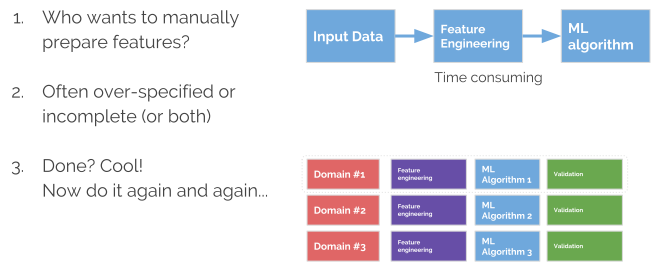
\includegraphics[width=0.8\linewidth,keepaspectratio]{dnlp11}

\tiny{(Ref:  A not-so-short introduction to Deep Learning NLP - Francesco Gadaleta, PhD)}
\end{center}

\end{frame}

%%%%%%%%%%%%%%%%%%%%%%%%%%%%%%%%%%%%%%%%%%%%%%%%%%%%%%%%%%%
\begin{frame}[fragile]\frametitle{Reasons for Applying Deep Learning to NLP}
Learning from unlabeled data

	\begin{itemize}
	\item Typical traditional Machine Leaning based NLP requires labeled training data.
	\item DL based methods like Skip Gram, CBOW generate word2vec by making labels from unlabeled data.
	\end{itemize}

\end{frame}


%%%%%%%%%%%%%%%%%%%%%%%%%%%%%%%%%%%%%%%%%%%%%%%%%%%%%%%%%%%
\begin{frame}[fragile]\frametitle{Reasons for Applying Deep Learning to NLP}
Human language is seqeuntial and contextual.

\begin{center}
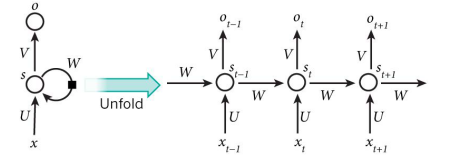
\includegraphics[width=0.8\linewidth,keepaspectratio]{dnlp12}

\tiny{(Ref:  A not-so-short introduction to Deep Learning NLP - Francesco Gadaleta, PhD)}
\end{center}

 RNNs serve the purpose well.
\end{frame}


%%%%%%%%%%%%%%%%%%%%%%%%%%%%%%%%%%%%%%%%%%%%%%%%%%%%%%%%%%%
\begin{frame}[fragile]\frametitle{Traditional NLP under threat?}
	\begin{itemize}
	\item Deep learning models have taken NLP by storm, achieving superior results across many applications.
	\item Many DL approaches do not model any  linguistic knowledge. They view language as a sequence of strings.
	\item Is this the end of NLP as a separate discipline?
	\end{itemize}

\end{frame}

%%%%%%%%%%%%%%%%%%%%%%%%%%%%%%%%%%%%%%%%%%%%%%%%%%%%%%%%%%%
\begin{frame}[fragile]\frametitle{NLP}
	\begin{itemize}
	\item Rule based systems (since 1960s): Regex
	\item   Machine Learning (since late 1980s): Naive Bayes, SVM, HMM
	\item Deep Learning (since 2000)
	\end{itemize}

\end{frame}


%%%%%%%%%%%%%%%%%%%%%%%%%%%%%%%%%%%%%%%%%%%%%%%%%%%%%%%%%%%
\begin{frame}[fragile]\frametitle{The Promise of Deep NLP }
\begin{center}
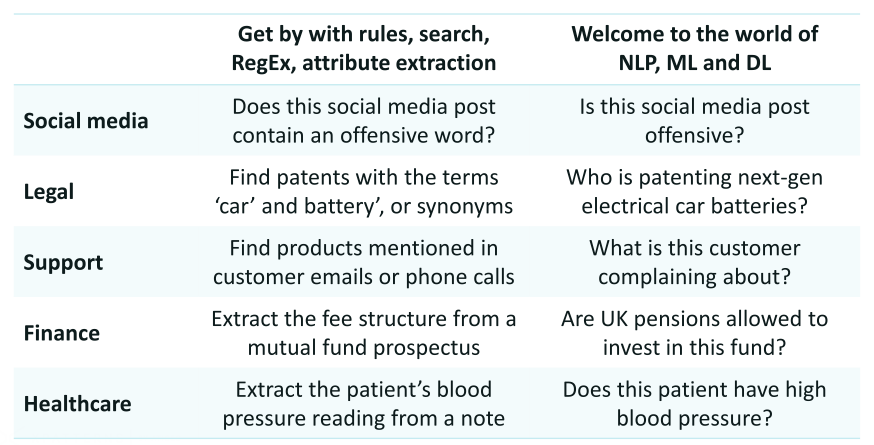
\includegraphics[width=\linewidth,keepaspectratio]{dnlp16}

\tiny{(Ref: Deep Learning for NLU - Dr. David Talby)}
\end{center}

\end{frame}


%%%%%%%%%%%%%%%%%%%%%%%%%%%%%%%%%%%%%%%%%%%%%%%%%%%%%%%%%%%
\begin{frame}[fragile]\frametitle{Deep NLP Opportunities}
\begin{center}
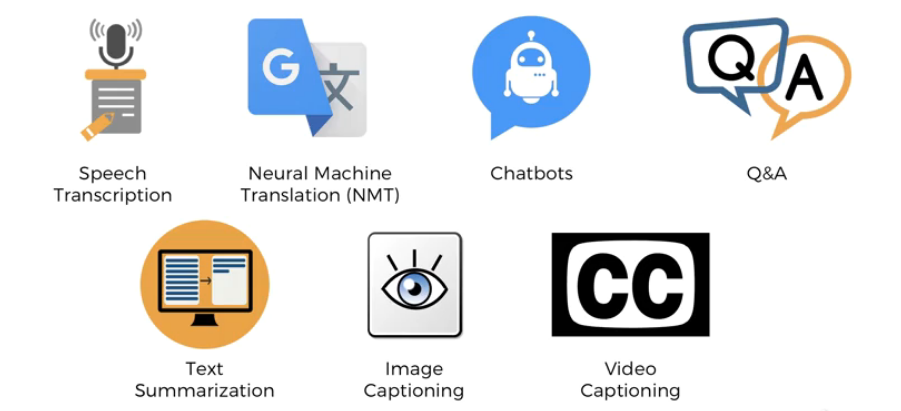
\includegraphics[width=\linewidth,keepaspectratio]{nlp3}

\tiny{(Ref: Deep Learning and NLP A-Z - Kirill Eremenko)}
\end{center}

\end{frame}

%%%%%%%%%%%%%%%%%%%%%%%%%%%%%%%%%%%%%%%%%%%%%%%%%%%%%%%%%%%
\begin{frame}
  \begin{center}
    {\Large Deep NLP Algorithms}
  \end{center}
\end{frame}


%%%%%%%%%%%%%%%%%%%%%%%%%%%%%%%%%%%%%%%%%%%%%%%%%%%%%%%%%%%
\begin{frame}[fragile]\frametitle{ LSTM for sequence labelling}
\begin{center}
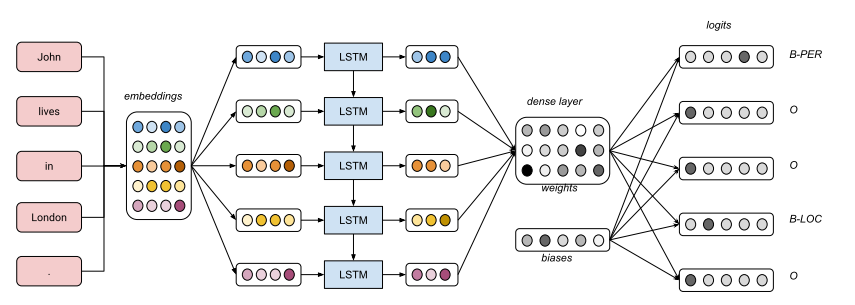
\includegraphics[width=\linewidth,keepaspectratio]{dnlp13}

\tiny{(Ref: Deep Learning for NLP - Yves Peirsman)}
\end{center}

Application: named entity recognition
\end{frame}

%%%%%%%%%%%%%%%%%%%%%%%%%%%%%%%%%%%%%%%%%%%%%%%%%%%%%%%%%%%
\begin{frame}[fragile]\frametitle{ Encoder-Decoder Architecture}
\begin{center}
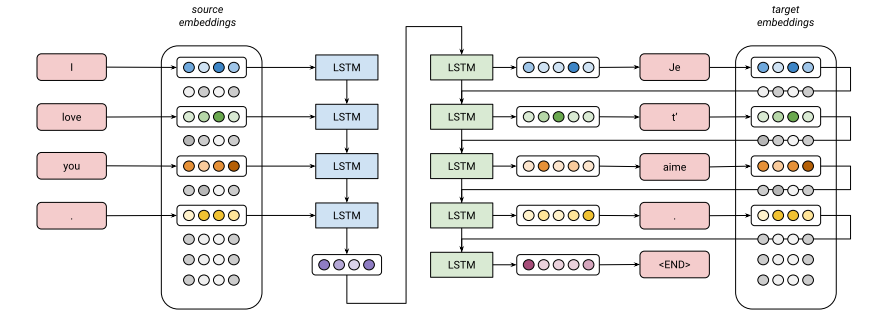
\includegraphics[width=\linewidth,keepaspectratio]{dnlp14}

\tiny{(Ref: Deep Learning for NLP - Yves Peirsman)}
\end{center}

Applications: machine translation, text summarization, dialogue modelling, etc
\end{frame}

%%%%%%%%%%%%%%%%%%%%%%%%%%%%%%%%%%%%%%%%%%%%%%%%%%%%%%%%%%%
\begin{frame}[fragile]\frametitle{Traditional Named Entity Recognition}
The problem
\begin{center}
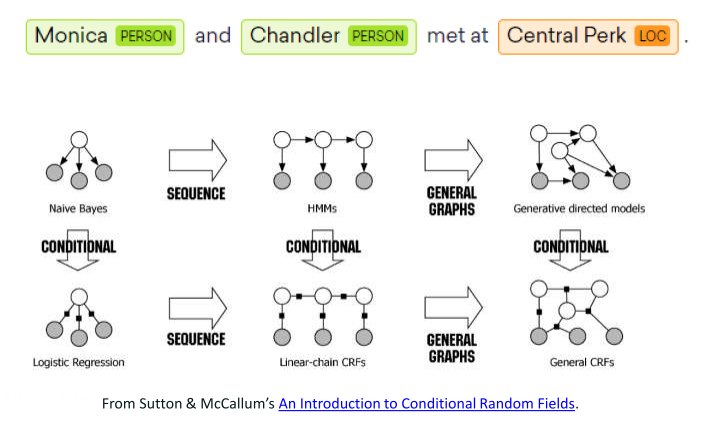
\includegraphics[width=\linewidth,keepaspectratio]{dnlp17}

\tiny{(Ref: Deep Learning for NLU - Dr. David Talby)}
\end{center}

\end{frame}

%%%%%%%%%%%%%%%%%%%%%%%%%%%%%%%%%%%%%%%%%%%%%%%%%%%%%%%%%%%
\begin{frame}[fragile]\frametitle{Traditional Named Entity Recognition}
Conditional Random Fields (CRFs), ``Classic'' machine learning approach

\begin{center}
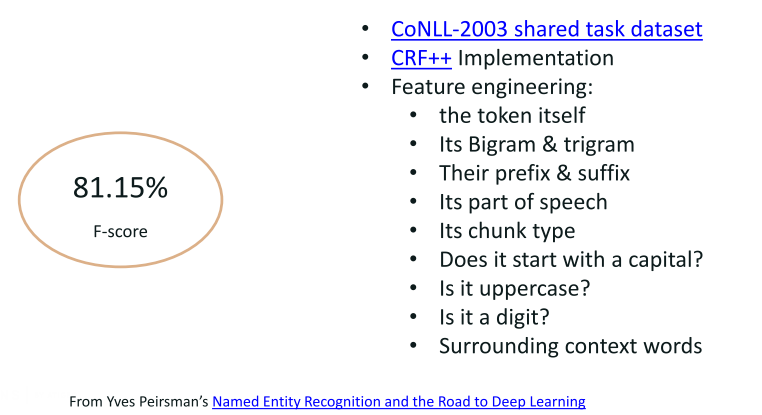
\includegraphics[width=\linewidth,keepaspectratio]{dnlp18}

\tiny{(Ref: Deep Learning for NLU - Dr. David Talby)}
\end{center}

\end{frame}

%%%%%%%%%%%%%%%%%%%%%%%%%%%%%%%%%%%%%%%%%%%%%%%%%%%%%%%%%%%
\begin{frame}[fragile]\frametitle{Deep Named Entity Recognition}
LSTM

\begin{center}
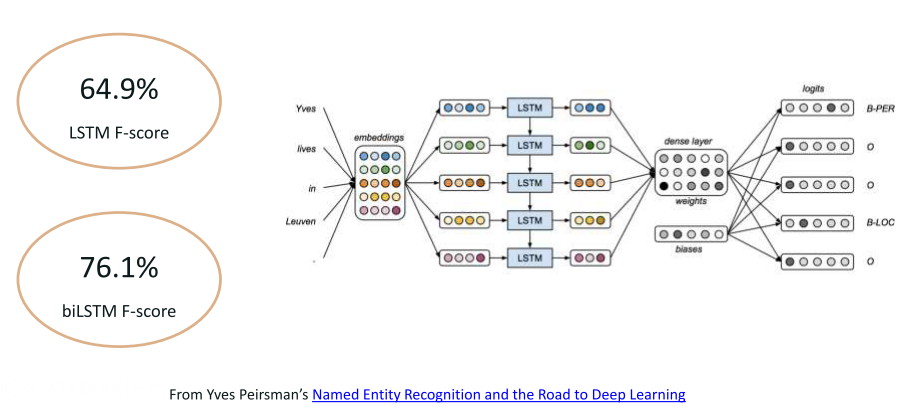
\includegraphics[width=\linewidth,keepaspectratio]{dnlp19}

\tiny{(Ref: Deep Learning for NLU - Dr. David Talby)}
\end{center}

\end{frame}

%%%%%%%%%%%%%%%%%%%%%%%%%%%%%%%%%%%%%%%%%%%%%%%%%%%%%%%%%%%
\begin{frame}[fragile]\frametitle{Deep Named Entity Recognition}
Bi-LSTM

\begin{center}
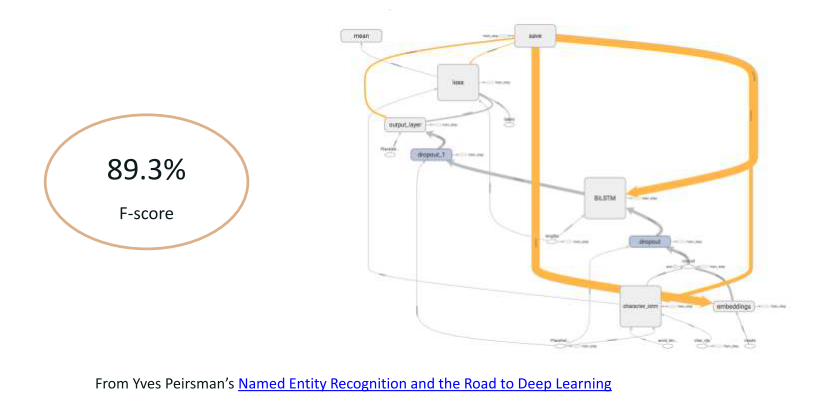
\includegraphics[width=\linewidth,keepaspectratio]{dnlp20}

\tiny{(Ref: Deep Learning for NLU - Dr. David Talby)}
\end{center}

\end{frame}



%%%%%%%%%%%%%%%%%%%%%%%%%%%%%%%%%%%%%%%%%%%%%%%%%%%%%%%%%%%
\begin{frame}[fragile]\frametitle{ Summary of DL algos for NLP}
\begin{center}
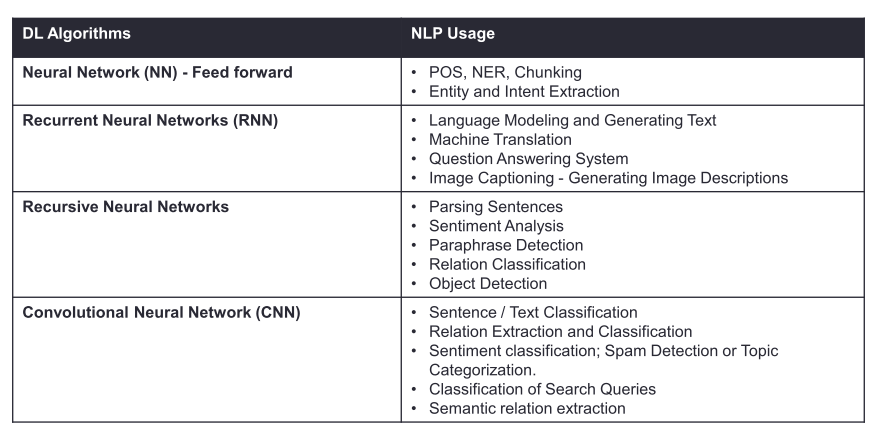
\includegraphics[width=\linewidth,keepaspectratio]{dnlp15}

\tiny{(Ref: Engineering Intelligent NLP Applications Using Deep Learning –  Part 2  Saurabh Kaushik)}
\end{center}


\end{frame}




%%%%%%%%%%%%%%%%%%%%%%%%%%%%%%%%%%%%%%%%%%%%%%%%%%%%%%%%%%%
\begin{frame}[fragile]\frametitle{Conclusion}
	\begin{itemize}
	\item Deep learning has simplified feature engineering in many cases (it certainly hasn't removed it) 
	\item Less feature engineering is leading to more complex machine learning architectures 
	\item Most of the time, these model architectures are as specific to a given task as feature engineering used to be.
	\item The job of the data scientist will stay sexy for a while (keep your fingers crossed on this one).
	\end{itemize}

\end{frame}

